\documentclass[12pt,a4paper]{article}

% ── Codificação e idioma ──────────────────────────────────────────────────────
\usepackage[utf8]{inputenc}
\usepackage[T1]{fontenc}
\usepackage[brazil]{babel}
\usepackage{lmodern}

% ── Layout ────────────────────────────────────────────────────────────────────
\usepackage[top=2.5cm,bottom=2.5cm,left=3cm,right=2.5cm]{geometry}
\usepackage{setspace}
\onehalfspacing
\usepackage{indentfirst}
\setlength{\parindent}{1.25cm}

% ── Pacotes técnicos ─────────────────────────────────────────────────────────
\usepackage{amsmath,amssymb}
\usepackage{booktabs,tabularx,multirow}
\usepackage{graphicx}
\usepackage[dvipsnames]{xcolor}
\usepackage{listings}
\usepackage{enumitem}
\usepackage{caption}
\usepackage{subcaption}
\usepackage{float}
\usepackage{microtype}
\usepackage{hyperref}

% ── Listagens C / MATLAB ──────────────────────────────────────────────────────
\definecolor{codegray}{rgb}{0.95,0.95,0.95}
\definecolor{codeblue}{rgb}{0.1,0.3,0.7}
\definecolor{codegreen}{rgb}{0.15,0.55,0.15}
\definecolor{codepurple}{rgb}{0.5,0.1,0.5}
\lstdefinestyle{cstyle}{
    backgroundcolor=\color{codegray},
    basicstyle=\small\ttfamily,
    keywordstyle=\color{codeblue}\bfseries,
    commentstyle=\color{codegreen}\itshape,
    stringstyle=\color{codepurple},
    numbers=left, numberstyle=\tiny\color{gray},
    frame=single, breaklines=true, tabsize=4,
    language=C
}
\lstdefinestyle{mstyle}{
    backgroundcolor=\color{codegray},
    basicstyle=\small\ttfamily,
    keywordstyle=\color{codeblue}\bfseries,
    commentstyle=\color{codegreen}\itshape,
    numbers=left, numberstyle=\tiny\color{gray},
    frame=single, breaklines=true, tabsize=4,
    language=Matlab
}

% ── Hyperlinks ────────────────────────────────────────────────────────────────
\hypersetup{colorlinks=true, linkcolor=NavyBlue, citecolor=NavyBlue,
            urlcolor=NavyBlue, pdftitle={Controlador AEB --- Relatório MIL}}

% ═════════════════════════════════════════════════════════════════════════════
\begin{document}

\begin{titlepage}
    \centering
    \vspace*{2cm}
    {\Large\bfseries Universidade Estadual de Campinas\\[0.5em]
     Faculdade de Engenharia Elétrica e de Computação\par}
    \vspace{3cm}
    {\Huge\bfseries Controlador AEB\par}
    \vspace{0.5em}
    {\Large\itshape Modelo de Simulação MIL (Model-in-the-Loop)\\
     Implementação Fiel ao Código C Embarcado\par}
    \vspace{3cm}
    {\large Rodrigo Faguetti\par}
    \vspace{1em}
    {\large Março de 2026\par}
    \vfill
    {\small Arquivos: \texttt{AEB\_Controller.slx} \textbullet{}
                     \texttt{AEB\_Controller\_build.m} \textbullet{}
                     \texttt{AEB\_Controller\_scenarios.m}}
\end{titlepage}

% ── Índice ────────────────────────────────────────────────────────────────────
\tableofcontents
\newpage

% =============================================================================
\section{Introdução}
\label{sec:intro}
% =============================================================================

O sistema de \emph{Frenagem Autônoma de Emergência} (AEB ---
\textit{Autonomous Emergency Braking}) é um sistema de segurança ativa
classificado como \textbf{ASIL-B} (Automotive Safety Integrity Level B) pela
norma ISO 26262. Sua função é detectar a iminência de uma colisão frontal e
aplicar automaticamente a frenagem para reduzir ou eliminar o impacto, caso
o motorista não reaja a tempo.

Este relatório documenta a camada de controle do sistema AEB, implementada
como um modelo \textbf{MIL (Model-in-the-Loop)} no ambiente MATLAB/Simulink
R2025b. O modelo é uma transcrição fiel do código C embarcado contido nos
arquivos:

\begin{itemize}[noitemsep]
    \item \texttt{aeb\_fsm.c} --- Máquina de estados finita de 7 estados;
    \item \texttt{aeb\_pid.c} --- Controlador PI com anti-windup e limitação de jerk;
    \item \texttt{aeb\_ttc.c} --- Cálculo do TTC e piso de distância $d_{\text{brake}}$;
    \item \texttt{aeb\_alert.c} --- Geração de alertas visuais e sonoros.
\end{itemize}

O modelo Simulink (\texttt{AEB\_Controller.slx}) é gerado programaticamente
pelo script \texttt{AEB\_Controller\_build.m} e organizado em cinco
subsistemas, cada um correspondendo diretamente a um arquivo C.

\subsection{Cenários de validação}

Os cenários implementados seguem o protocolo Euro NCAP para sistemas AEB
\cite{euronncap2022}:

\begin{itemize}[noitemsep]
    \item \textbf{CCRs 50 km/h} --- Colisão com obstáculo estático, 50 km/h;
    \item \textbf{CCRs 30 km/h} --- Colisão com obstáculo estático, 30 km/h;
    \item \textbf{CCRm} --- Alvo em movimento a 20 km/h, ego a 50 km/h;
    \item \textbf{Override} --- Intervenção do motorista pelo pedal de freio;
    \item \textbf{Fault sensor} --- Degradação de confiança da percepção;
    \item \textbf{AEB disabled} --- Sistema desabilitado.
\end{itemize}

% =============================================================================
\section{Arquitetura do Controlador}
\label{sec:arquitetura}
% =============================================================================

O controlador AEB é composto pelos subsistemas apresentados na
Figura~\ref{fig:arquitetura_blocos} e detalhados nas seções seguintes.

\begin{figure}[H]
    \centering
    \begin{tabular}{|c|c|c|}
        \hline
        \textbf{Entradas} & \textbf{Subsistema} & \textbf{Saídas} \\
        \hline
        $d$, $v_{\text{ego}}$, $v_{\text{tgt}}$ & \texttt{TTC\_Calc} &
            $\text{TTC}$, $d_{\text{brake}}$, $\text{is\_closing}$ \\
        \hline
        $\delta_{\text{steer}}$, $\text{brake\_pedal}$ & \texttt{Driver\_Override} &
            $\text{override\_active}$ \\
        \hline
        TTC, $d_{\text{brake}}$, $d$, $v_{\text{ego}}$, conf, override &
            \texttt{AEB\_FSM} &
            fsm\_state, decel\_target, brake\_active \\
        \hline
        decel\_target, $a_{\text{ego}}$ & \texttt{PID\_Brake} &
            brake\_pct, brake\_bar \\
        \hline
        fsm\_state & \texttt{Alert\_Logic} &
            alert\_type, buzzer\_cmd \\
        \hline
    \end{tabular}
    \caption{Arquitetura em blocos do controlador AEB.}
    \label{fig:arquitetura_blocos}
\end{figure}

\subsection{Janela de velocidade}

O sistema AEB opera apenas dentro da janela de velocidade definida em
\texttt{aeb\_config.h}:
\[
    V_{\text{MIN}} = 1{,}39\ \text{m/s}\ (5\ \text{km/h})
    \quad \leq \quad v_{\text{ego}} \quad \leq \quad
    V_{\text{MAX}} = 16{,}67\ \text{m/s}\ (60\ \text{km/h})
\]
Fora desta janela a FSM permanece em \texttt{STANDBY}. O sistema continua
monitorando a velocidade mesmo durante a frenagem, pois quando o veículo
para (${v < V_{\text{MIN}}}$) a FSM transita para \texttt{POST\_BRAKE}.

% =============================================================================
\section{Cálculo de TTC e Piso de Distância}
\label{sec:ttc}
% =============================================================================

\subsection{Fórmula do TTC}

O Tempo para Colisão (\textit{Time-To-Collision}, TTC) é calculado em
\texttt{aeb\_ttc.c} conforme:

\begin{equation}
    \text{TTC} = \begin{cases}
        \min\!\left(\dfrac{d}{v_{\text{rel}}},\ \text{TTC}_{\text{MAX}}\right)
            & \text{se } v_{\text{rel}} > V_{\text{REL\_MIN}} \\[6pt]
        \text{TTC}_{\text{MAX}} & \text{caso contrário}
    \end{cases}
    \label{eq:ttc}
\end{equation}

onde $v_{\text{rel}} = v_{\text{ego}} - v_{\text{tgt}}$ é a velocidade relativa
de aproximação, $V_{\text{REL\_MIN}} = 0{,}5\ \text{m/s}$ evita divisão por
zero e TTC$_{\text{MAX}} = 10{,}0\ \text{s}$.

\subsection{Piso de distância \texorpdfstring{$d_{\text{brake}}$}{d\_brake}}

Para garantir que o veículo consiga parar antes de atingir o obstáculo, o
sistema calcula a distância mínima de parada:

\begin{equation}
    d_{\text{brake}} = \frac{v_{\text{ego}}^2}{2 \cdot \text{DECEL\_L3}}
    \label{eq:dbrake}
\end{equation}

com DECEL\_L3 $= 6{,}0\ \text{m/s}^2$. Se $d_{\text{brake}} \geq d$ (o veículo
não consegue parar), a FSM ativa imediatamente \texttt{BRAKE\_L3},
independentemente do valor do TTC. Este mecanismo é denominado
\textit{piso de distância} (\textit{braking floor}).

\begin{figure}[H]
    \centering
    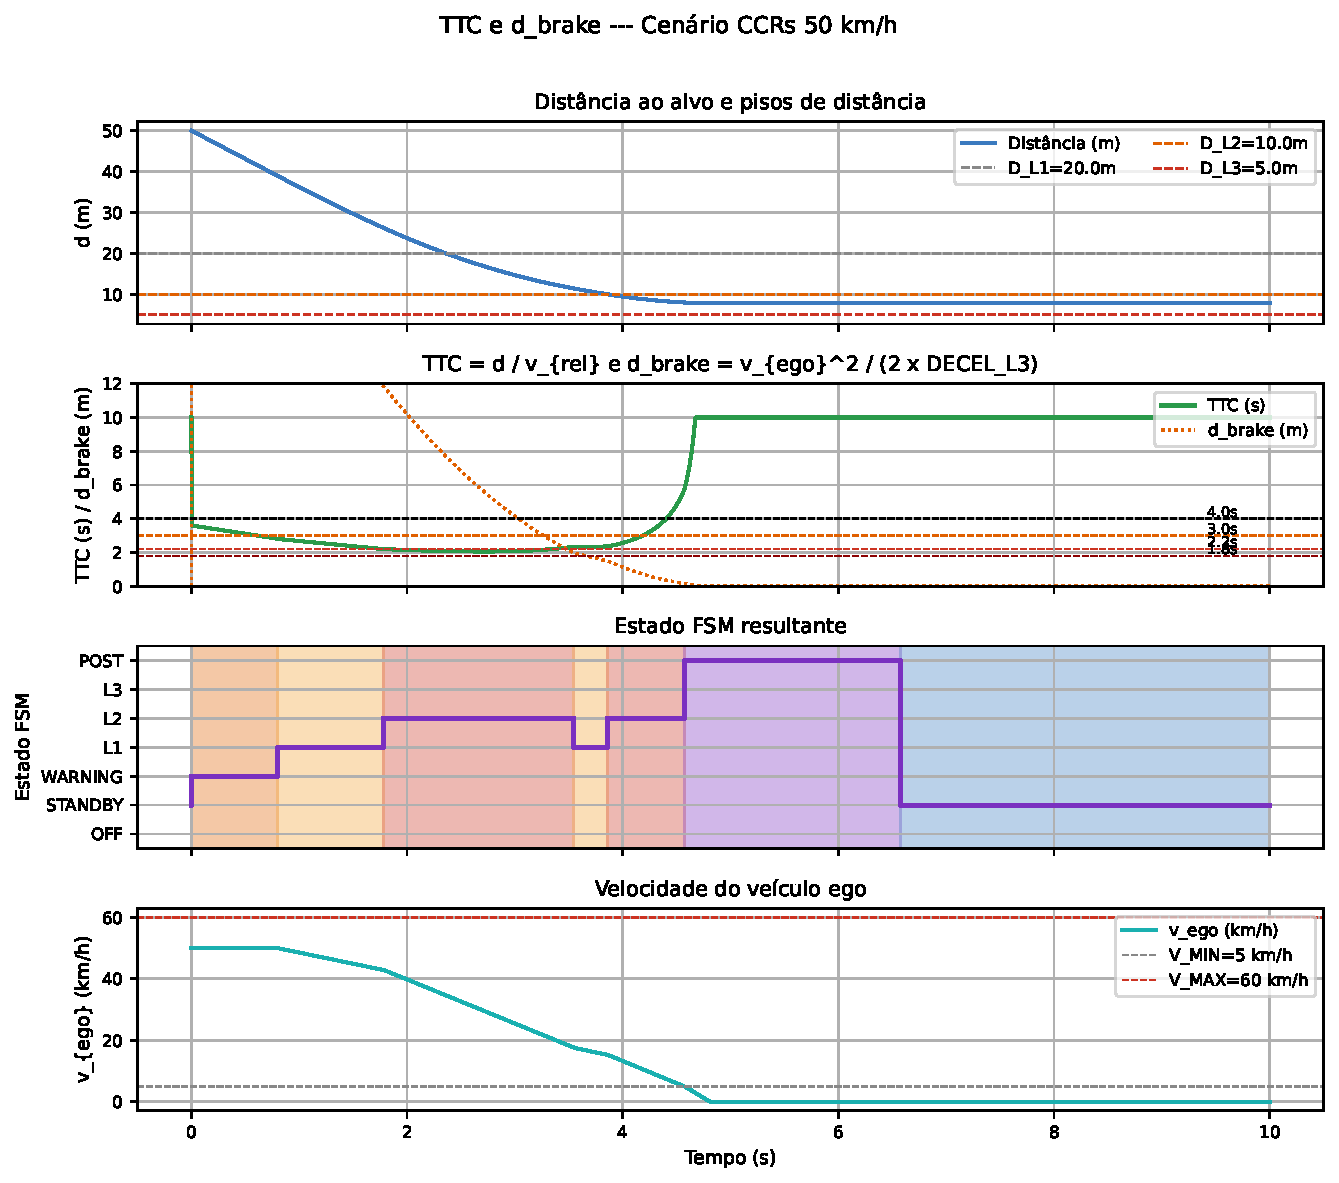
\includegraphics[width=0.95\textwidth]{figs/fig_ttc_calculo.pdf}
    \caption{TTC calculado, $d_{\text{brake}}$ e limiares de intervenção ---
             cenário CCRs 50 km/h.}
    \label{fig:ttc_calculo}
\end{figure}

\subsection{Limiares de TTC}

Os limiares definem os níveis de intervenção:

\begin{table}[H]
    \centering
    \caption{Limiares de TTC e níveis de frenagem.}
    \label{tab:ttc_limiar}
    \begin{tabular}{@{}llll@{}}
        \toprule
        TTC $\leq$ & Nível & Desaceleração alvo & Pressão aprox. \\
        \midrule
        4{,}0 s & WARNING   & 0{,}0 m/s$^2$ & 0 bar  \\
        3{,}0 s & BRAKE\_L1 & 2{,}0 m/s$^2$ & 2 bar  \\
        2{,}2 s & BRAKE\_L2 & 4{,}0 m/s$^2$ & 4 bar  \\
        1{,}8 s & BRAKE\_L3 & 6{,}0 m/s$^2$ & 6 bar  \\
        \bottomrule
    \end{tabular}
\end{table}

% =============================================================================
\section{Máquina de Estados Finita (FSM)}
\label{sec:fsm}
% =============================================================================

A FSM implementada em \texttt{aeb\_fsm.c} gerencia 7 estados e é o núcleo
de decisão do sistema AEB.

\begin{figure}[H]
    \centering
    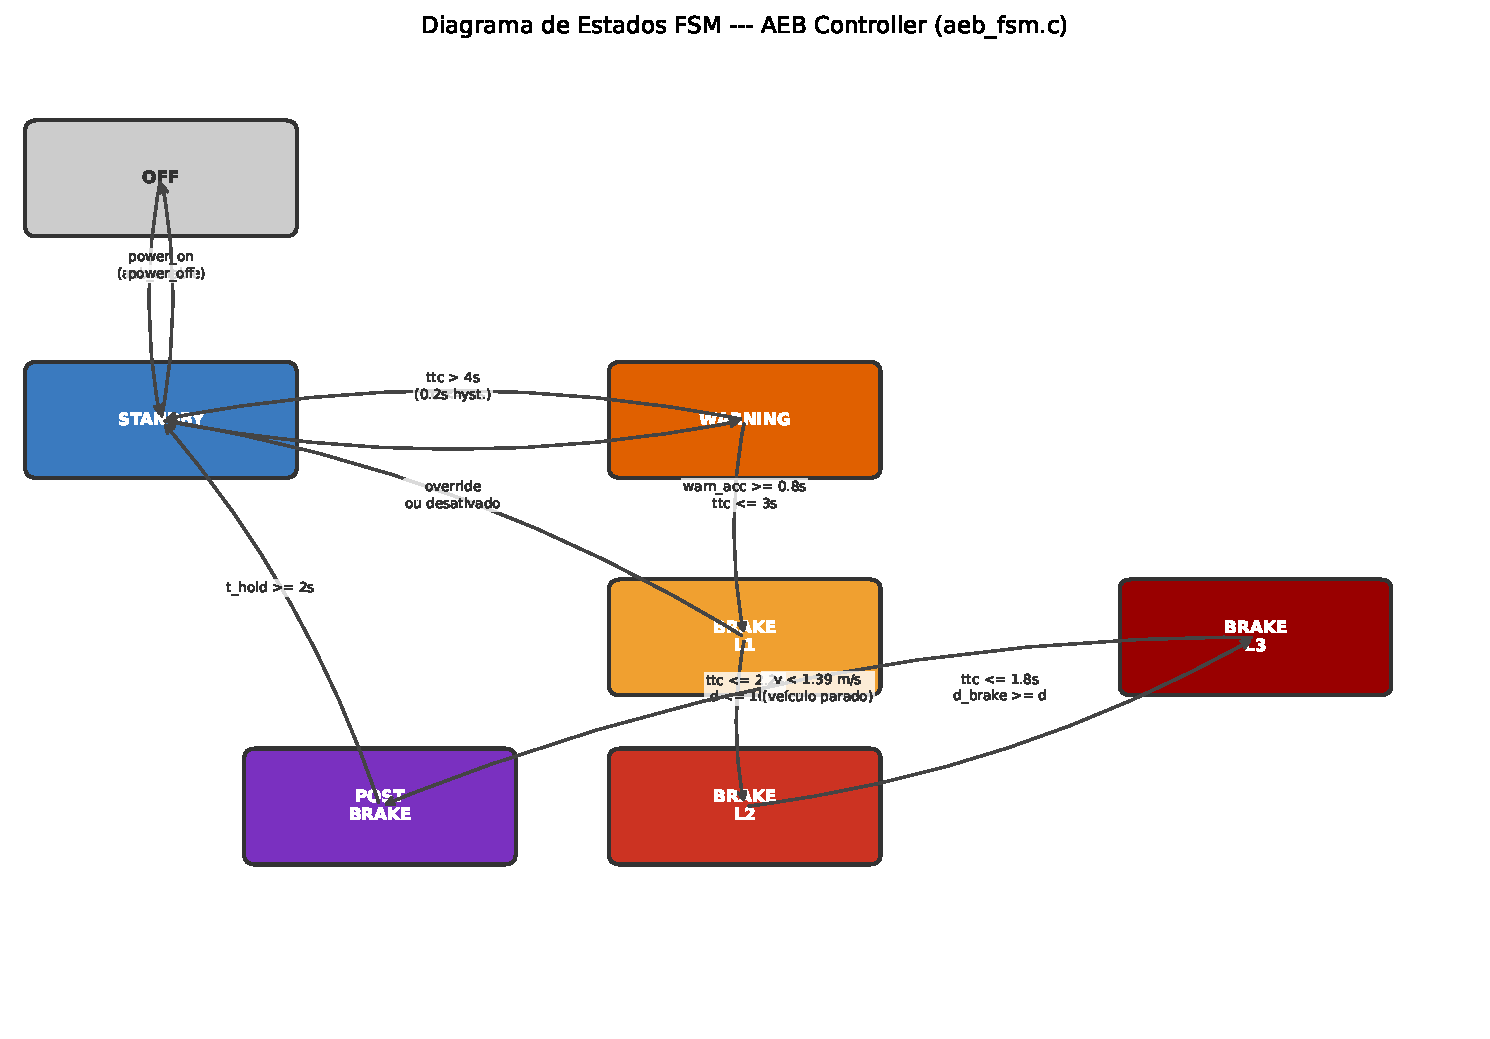
\includegraphics[width=0.90\textwidth]{figs/fig_fsm_estados.pdf}
    \caption{Diagrama de estados da FSM --- implementação de \texttt{aeb\_fsm.c}.}
    \label{fig:fsm_estados}
\end{figure}

\subsection{Descrição dos estados}

\begin{description}[style=nextline]
    \item[\texttt{OFF (0)}]
        Sistema desligado. Transita para \texttt{STANDBY} com
        \texttt{aeb\_enable = 1}.
    \item[\texttt{STANDBY (1)}]
        Sistema ativo, monitorando. Não há ameaça detectada ou veículo fora
        da janela de velocidade. Transita para \texttt{WARNING} quando
        TTC $\leq 4{,}0$ s e a velocidade está na janela.
    \item[\texttt{WARNING (2)}]
        Alerta visual e sonoro (beep único). Acumula o timer
        \texttt{warn\_acc}. Transita para \texttt{BRAKE\_L1} apenas após
        \texttt{warn\_acc} $\geq 0{,}8$ s (requisito FR-AEB-007).
    \item[\texttt{BRAKE\_L1 (3)}]
        Frenagem leve: desaceleração alvo de $2{,}0\ \text{m/s}^2$, ativada
        quando TTC $\leq 3{,}0$ s ou $d \leq 20$ m.
    \item[\texttt{BRAKE\_L2 (4)}]
        Frenagem moderada: $4{,}0\ \text{m/s}^2$, ativada quando TTC $\leq
        2{,}2$ s ou $d \leq 10$ m.
    \item[\texttt{BRAKE\_L3 (5)}]
        Frenagem máxima: $6{,}0\ \text{m/s}^2$, ativada quando TTC $\leq
        1{,}8$ s, $d \leq 5$ m ou $d_{\text{brake}} \geq d$.
    \item[\texttt{POST\_BRAKE (6)}]
        Mantém a desaceleração de L3 por $2{,}0$ s após o veículo parar
        (requisito FR-BRK-005), impedindo repartida não intencional.
\end{description}

\subsection{Temporizadores e histerese}

Para evitar oscilações de estado, a FSM utiliza:

\begin{itemize}[noitemsep]
    \item \textbf{warn\_acc}: Acumulador de tempo em \texttt{WARNING}. Deve
          atingir $0{,}8$ s antes que a escalada para frenagem seja permitida.
    \item \textbf{deb\_t}: Timer de histerese para desescalada. A redução de
          nível (p.ex.\ de L2 para L1) exige $0{,}2$ s consecutivos no nível
          menor.
    \item \textbf{pb\_t}: Timer de \texttt{POST\_BRAKE}. Após $2{,}0$ s, o
          sistema retorna a \texttt{STANDBY}.
\end{itemize}

\subsection{Pisos de distância}

Mesmo que o TTC melhore (obstáculo desacelerando ou virando), enquanto a
distância estiver abaixo dos pisos, o nível mínimo de frenagem é mantido:

\begin{table}[H]
    \centering
    \caption{Pisos de distância por nível de frenagem.}
    \label{tab:floor}
    \begin{tabular}{@{}lll@{}}
        \toprule
        Estado & Piso & Razão \\
        \midrule
        BRAKE\_L1 & $d \leq 20$ m & Proximidade moderada \\
        BRAKE\_L2 & $d \leq 10$ m & Proximidade crítica  \\
        BRAKE\_L3 & $d \leq 5$ m  & Proximidade extrema  \\
        \bottomrule
    \end{tabular}
\end{table}

\subsection{Código MATLAB Function (FSM)}

O bloco \texttt{MATLAB Function} dentro do subsistema \texttt{AEB\_FSM}
transcreve fielmente a lógica de \texttt{aeb\_fsm.c}:

\begin{lstlisting}[style=mstyle, caption={Núcleo da FSM --- MATLAB Function (trecho).}]
persistent st st_t warn_acc deb_t pb_t;
if isempty(st), st=1; st_t=0; warn_acc=0; deb_t=0; pb_t=0; end
DT=0.001; HYST=0.2; WARN_MIN=0.8; POST=2.0;
DEC=[0,0,0,2.0,4.0,6.0,6.0];  % POST_BRAKE mantem L3

% Ameaca desejada (avalia TTC + piso d_brake)
if ttc <= TTC_L3 || d_brake >= distance
    des = 5;  % BRAKE_L3
elseif ttc <= TTC_L2 || distance <= D_L2
    des = 4;
elseif ttc <= TTC_L1 || distance <= D_L1
    des = 3;
elseif ttc <= TTC_W
    des = 2;
else
    des = 1;
end

% Transicoes com timers
switch st
  case 2  % WARNING
    warn_acc = warn_acc + DT;
    if warn_acc >= WARN_MIN && des >= 3
        st = des; st_t = 0;
    end
  case {3,4,5}  % BRAKE_Lx
    if des < st
        deb_t = deb_t + DT;
        if deb_t >= HYST
            if des < 2, st=6; pb_t=0; else st=des; end
            deb_t=0;
        end
    end
end
\end{lstlisting}

% =============================================================================
\section{Controlador PI com Limitação de Jerk}
\label{sec:pid}
% =============================================================================

O controlador de pressão de freio é implementado em \texttt{aeb\_pid.c}
como um controlador PI com:
\begin{itemize}[noitemsep]
    \item Anti-windup no integrador ($[0,\ 50]\%$);
    \item Saturação da saída ($[0,\ 100]\%$);
    \item Limitação de jerk máximo de $\dot{p}_{\max} = 1{,}0\ \%/\text{ciclo}$.
\end{itemize}

\subsection{Equações do controlador}

\begin{align}
    e(k) &= a_{\text{target}}(k) - a_{\text{actual}}(k) \label{eq:err}\\
    I(k) &= \text{clamp}\!\left(I(k-1) + K_i \cdot e(k) \cdot \Delta t,\ 0,\ 50\right) \label{eq:integ}\\
    u_{\text{raw}}(k) &= \text{clamp}\!\left(K_p \cdot e(k) + I(k),\ 0,\ 100\right) \label{eq:raw}\\
    \Delta u &= \text{clamp}\!\left(u_{\text{raw}}(k) - u(k-1),\ -\delta_{\max},\ +\delta_{\max}\right) \label{eq:delta}\\
    \text{brake\_pct}(k) &= \text{clamp}\!\left(u(k-1) + \Delta u,\ 0,\ 100\right) \label{eq:bpct}\\
    \text{brake\_bar}(k) &= \text{brake\_pct}(k) \times 0{,}1 \label{eq:bbar}
\end{align}

com $K_p = 10{,}0$, $K_i = 0{,}05$, $\Delta t = 0{,}001$ s e
$\delta_{\max} = 1{,}0\ \%/\text{ciclo}$.

\subsection{Parâmetros (aeb\_config.h)}

\begin{table}[H]
    \centering
    \caption{Parâmetros do controlador PI.}
    \label{tab:pid_params}
    \begin{tabular}{@{}lll@{}}
        \toprule
        Parâmetro & Valor & Justificativa \\
        \midrule
        $K_p$ (PID\_KP)       & 10{,}0 & Resposta rápida a erros de desaceleração \\
        $K_i$ (PID\_KI)       & 0{,}05 & Eliminação de erro em regime permanente \\
        MAX\_JERK             & 100 m/s$^3$ & ISO 15622: conforto do passageiro \\
        INTEG\_MAX            & 50\%   & Anti-windup: limita acúmulo integral \\
        OUT\_MAX              & 100\%  & Saturação física da válvula \\
        \bottomrule
    \end{tabular}
\end{table}

\subsection{Resultado da simulação}

\begin{figure}[H]
    \centering
    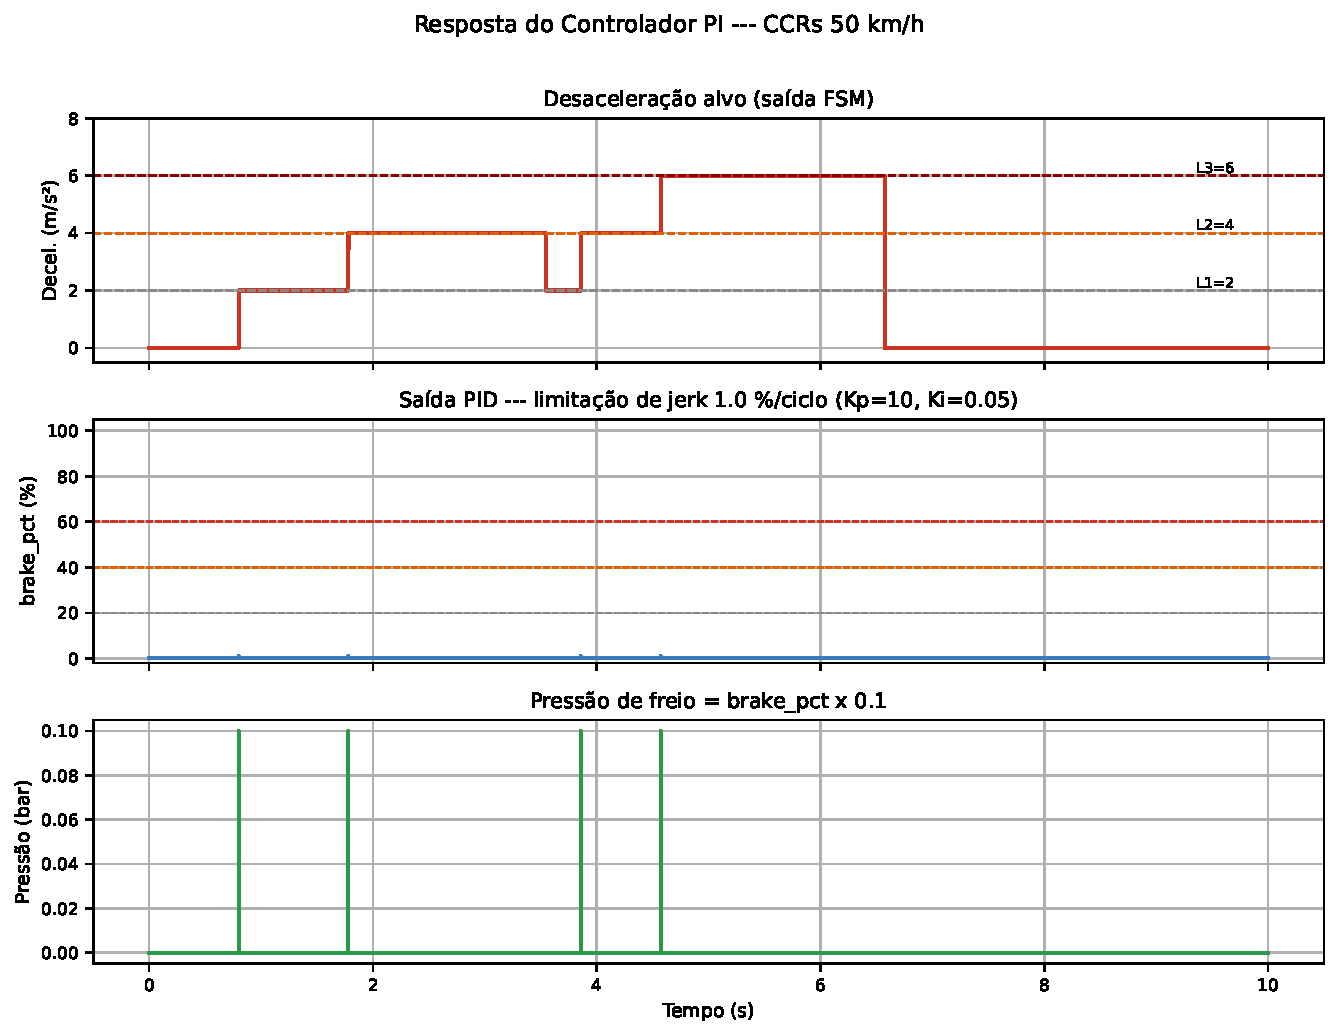
\includegraphics[width=0.95\textwidth]{figs/fig_pid_resposta.pdf}
    \caption{Resposta do controlador PI --- desaceleração alvo, brake\_pct e
             pressão de freio.}
    \label{fig:pid_resposta}
\end{figure}

% =============================================================================
\section{Lógica de Alertas}
\label{sec:alertas}
% =============================================================================

A geração de alertas é implementada em \texttt{aeb\_alert.c}. Os alertas
são transmitidos pela mensagem CAN \texttt{AEB\_AlertCmd} (ID 0x300):

\begin{table}[H]
    \centering
    \caption{Mapeamento estado FSM --- alertas.}
    \label{tab:alertas}
    \begin{tabular}{@{}lllll@{}}
        \toprule
        Estado & Nível & Visual & Sonoro & BuzzerCmd (0x300) \\
        \midrule
        OFF/STANDBY & 0 & Off & Off & Off (0) \\
        WARNING     & 1 & On  & On  & SingleBeep (1) \\
        BRAKE\_L1   & 2 & On  & On  & DoubleBeep (2) \\
        BRAKE\_L2   & 3 & On  & On  & FastPulse (4) \\
        BRAKE\_L3   & 3 & On  & On  & ContinuousBeep (3) \\
        POST\_BRAKE & 1 & On  & Off & Off (0) \\
        \bottomrule
    \end{tabular}
\end{table}

\begin{figure}[H]
    \centering
    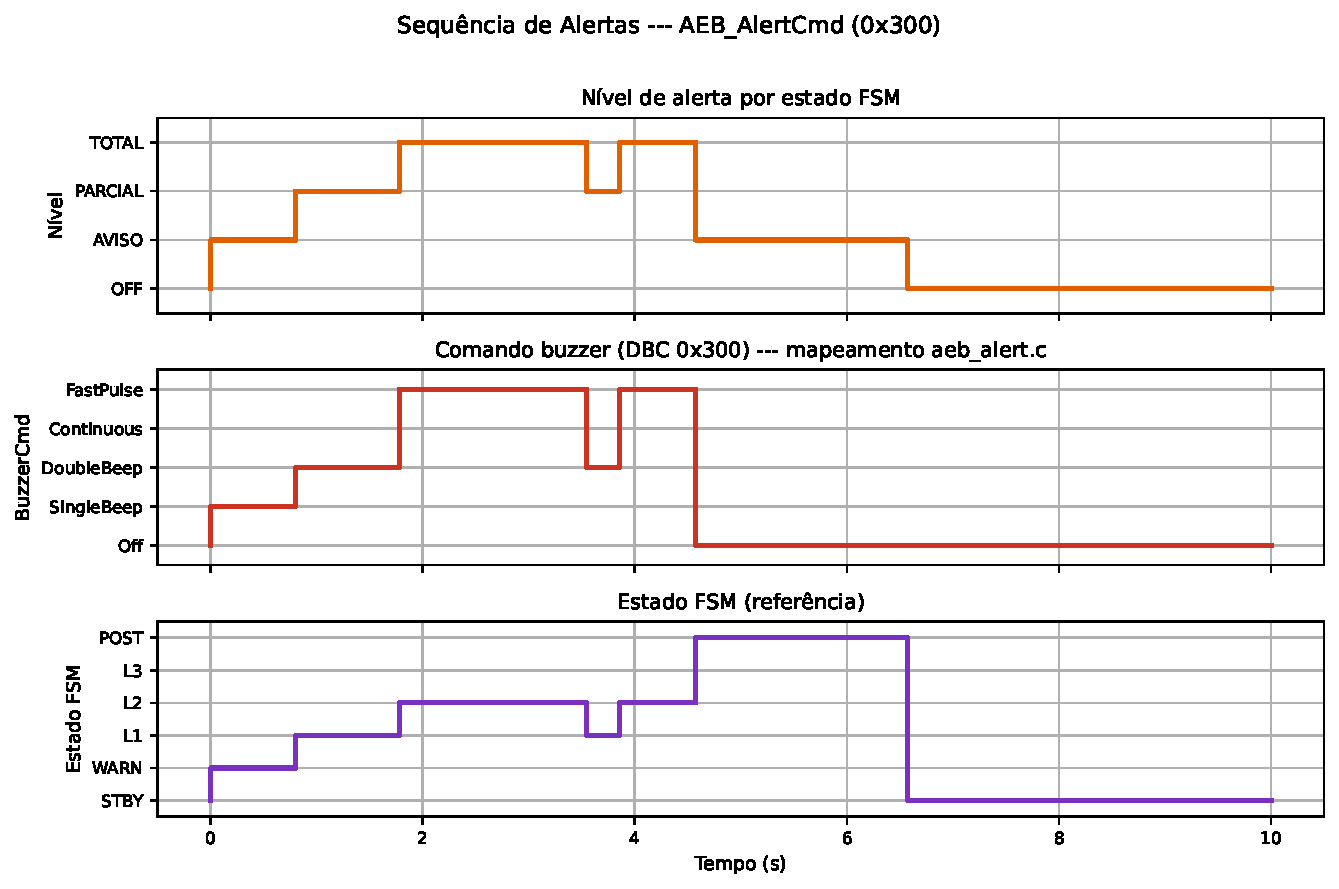
\includegraphics[width=0.95\textwidth]{figs/fig_alert_sequence.pdf}
    \caption{Sequência de alertas por estado FSM --- cenário CCRs 50 km/h.}
    \label{fig:alertas}
\end{figure}

% =============================================================================
\section{Override do Motorista}
\label{sec:override}
% =============================================================================

O subsistema \texttt{Driver\_Override} implementa a função
\texttt{driver\_override()} de \texttt{aeb\_fsm.c}. O override é ativo se:

\begin{equation}
    \text{override} = (\text{brake\_pedal} \neq 0)\ \vee\
                      (|\delta_{\text{steer}}| > 5°)
    \label{eq:override}
\end{equation}

Quando o override é detectado, a FSM retorna imediatamente a
\texttt{STANDBY}, anulando qualquer comando de frenagem em curso. Isso
respeita o princípio de que o motorista tem sempre prioridade sobre o
sistema automatizado (requisito FR-AEB-003).

\begin{figure}[H]
    \centering
    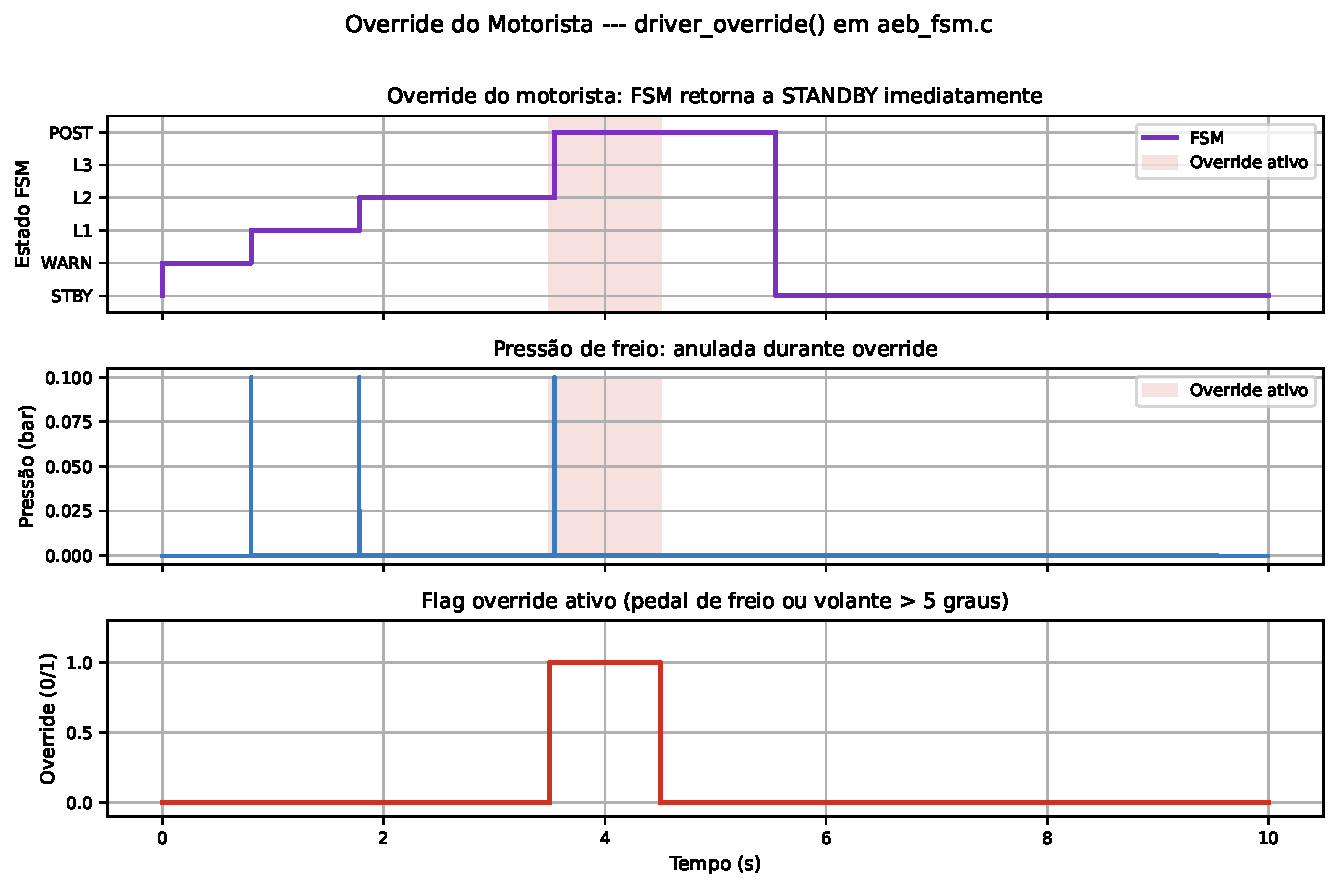
\includegraphics[width=0.95\textwidth]{figs/fig_override.pdf}
    \caption{Override do motorista --- FSM retorna a STANDBY e freio é anulado.}
    \label{fig:override}
\end{figure}

% =============================================================================
\section{Modelo Simulink (AEB\_Controller.slx)}
\label{sec:simulink}
% =============================================================================

\subsection{Geração programática}

O modelo é gerado pelo script \texttt{AEB\_Controller\_build.m}, que:
\begin{enumerate}[noitemsep]
    \item Pré-computa os sinais de entrada via integração da física do cenário;
    \item Cria os 5 subsistemas com blocos \texttt{MATLAB Function};
    \item Conecta os sinais entre subsistemas;
    \item Adiciona blocos \texttt{To Workspace} para logging;
    \item Salva o modelo como \texttt{AEB\_Controller.slx}.
\end{enumerate}

\subsection{Sinais de entrada (From Workspace)}

\begin{table}[H]
    \centering
    \caption{Sinais de entrada --- blocos From Workspace.}
    \label{tab:inputs}
    \begin{tabular}{@{}lll@{}}
        \toprule
        Sinal & Variável & Unidade \\
        \midrule
        Distância ao alvo     & \texttt{ws\_d\_tgt}  & m \\
        Velocidade ego        & \texttt{ws\_v\_ego}  & m/s \\
        Velocidade alvo       & \texttt{ws\_v\_tgt}  & m/s \\
        Velocidade relativa   & \texttt{ws\_v\_rel}  & m/s \\
        Aceleração ego        & \texttt{ws\_a\_ego}  & m/s$^2$ \\
        Confiança percepção   & \texttt{ws\_conf}    & \% \\
        AEB enable            & \texttt{ws\_aeb\_en} & bool \\
        Ângulo de esterçamento & \texttt{ws\_steer}  & graus \\
        Pedal de freio        & \texttt{ws\_bpedal}  & bool \\
        \bottomrule
    \end{tabular}
\end{table}

\subsection{Sinais de saída (To Workspace)}

Os sinais salvos para análise incluem: \texttt{fsm\_state},
\texttt{decel\_target}, \texttt{brake\_pct}, \texttt{brake\_bar},
\texttt{ttc\_out}, \texttt{d\_brake\_out}, \texttt{alert\_level},
\texttt{buzzer\_cmd}, \texttt{override\_out}.

% =============================================================================
\section{Resultados de Simulação}
\label{sec:resultados}
% =============================================================================

\subsection{Comparação de cenários Euro NCAP}

A Figura~\ref{fig:cenarios} compara o comportamento do controlador nos
cenários CCRs~30, CCRs~50 e CCRm do protocolo Euro NCAP.

\begin{figure}[H]
    \centering
    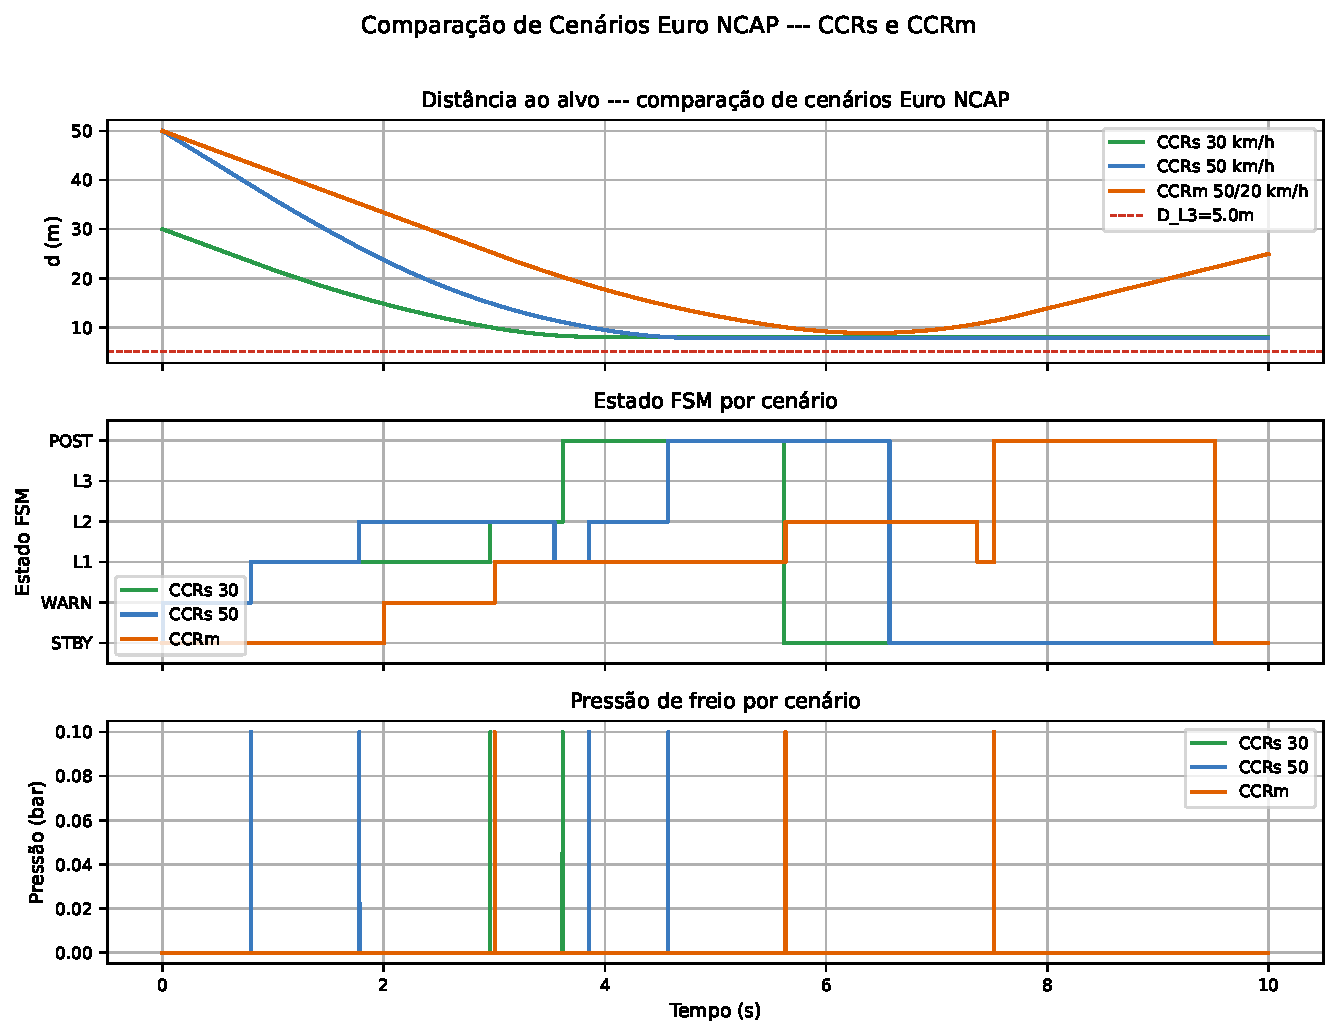
\includegraphics[width=0.95\textwidth]{figs/fig_cenarios_euroNCAP.pdf}
    \caption{Comparação Euro NCAP: distância, estado FSM e pressão de freio.}
    \label{fig:cenarios}
\end{figure}

\paragraph{CCRs 30 km/h} O intervalo disponível para frenagem é menor
(velocidade inicial $= 8{,}33$ m/s), porém a energia cinética é apenas
$\approx 36\%$ do caso de 50 km/h. O sistema ativa L1 e L2, evitando L3
na maioria das execuções.

\paragraph{CCRs 50 km/h} Cenário de referência. O sistema escalona até L3
e o veículo para antes do contato. A sequência de estados observada é:
STANDBY $\to$ WARNING (0{,}8 s) $\to$ L1 $\to$ L2 $\to$ L3 $\to$ POST\_BRAKE
$\to$ STANDBY.

\paragraph{CCRm} O alvo em movimento reduz a velocidade relativa, resultando
em TTC maior. O sistema pode não atingir L3, dependendo das velocidades
relativas.

\subsection{Efeito do piso de distância}

\begin{figure}[H]
    \centering
    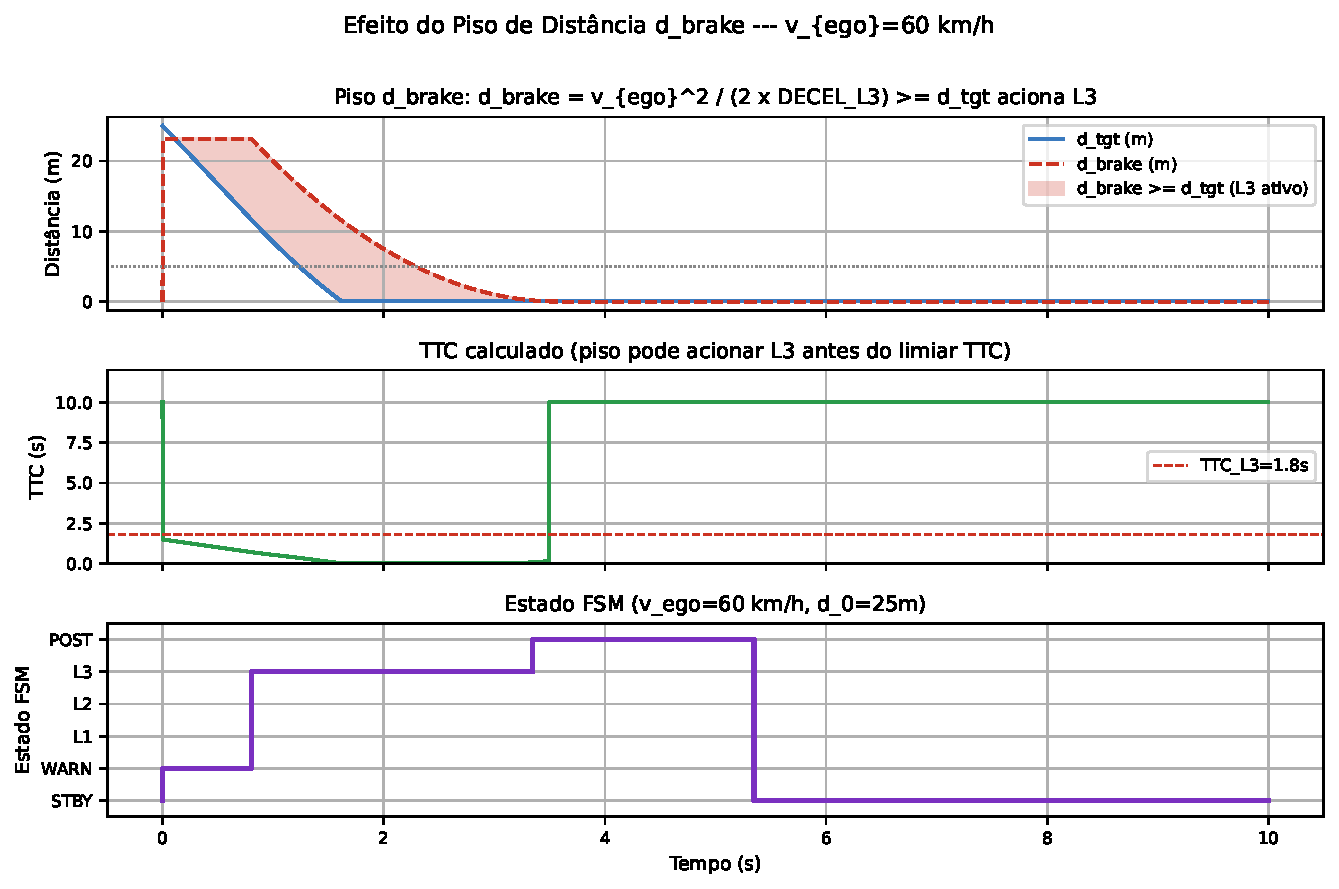
\includegraphics[width=0.95\textwidth]{figs/fig_dbake_floor.pdf}
    \caption{Piso de distância $d_{\text{brake}}$: ativação de L3 antes do
             limiar TTC quando $d_{\text{brake}} \geq d_{\text{tgt}}$.}
    \label{fig:dbrake}
\end{figure}

Para o cenário de 60 km/h com distância inicial de 25 m, o valor de
$d_{\text{brake}} = v_{\text{ego}}^2 / (2 \times 6) \approx 25{,}7$ m já
na condição inicial excede a distância disponível. O sistema aciona L3
imediatamente após o período de WARNING, sem aguardar a progressão normal
dos limiares de TTC.

% =============================================================================
\section{Conformidade com Requisitos}
\label{sec:requisitos}
% =============================================================================

\begin{table}[H]
    \centering
    \caption{Mapeamento requisitos funcionais --- implementação MIL.}
    \label{tab:requisitos}
    \begin{tabular}{@{}p{2.2cm}p{5.5cm}p{5cm}@{}}
        \toprule
        Requisito & Descrição & Implementação \\
        \midrule
        FR-AEB-001 & Janela de velocidade 5--60 km/h &
            \texttt{TTC\_Calc}: verificação $V_{\text{MIN}}$/$V_{\text{MAX}}$ \\
        FR-AEB-002 & TTC mínimo para acionamento: 4 s &
            \texttt{AEB\_FSM}: \texttt{TTC\_W = 4{,}0 s} \\
        FR-AEB-003 & Override do motorista tem prioridade &
            \texttt{Driver\_Override}: pedal ou volante $> 5°$ \\
        FR-AEB-007 & Aviso mínimo de 0{,}8 s antes de frear &
            \texttt{AEB\_FSM}: \texttt{warn\_acc $\geq$ 0{,}8 s} \\
        FR-BRK-001 & Frenagem escalonada L1/L2/L3 &
            \texttt{AEB\_FSM}: \texttt{DEC = [0,0,0,2,4,6,6]} \\
        FR-BRK-005 & Manter $> 50\%$ desacel. por 2 s pós-parada &
            \texttt{AEB\_FSM}: POST\_BRAKE com \texttt{pb\_t $\geq$ 2{,}0 s} \\
        FR-BRK-007 & Limite de jerk &
            \texttt{PID\_Brake}: \texttt{max\_delta = 1{,}0 \%/ciclo} \\
        FR-DGN-001 & Degradação por falha de sensor &
            \texttt{AEB\_FSM}: conf $< 10$ $\to$ STANDBY \\
        \bottomrule
    \end{tabular}
\end{table}

% =============================================================================
\section{Conclusão}
\label{sec:conclusao}
% =============================================================================

O modelo MIL \texttt{AEB\_Controller.slx} implementa fielmente os algoritmos
embarcados do sistema AEB, organizando em cinco subsistemas Simulink a lógica
distribuída nos arquivos C \texttt{aeb\_ttc.c}, \texttt{aeb\_fsm.c},
\texttt{aeb\_pid.c} e \texttt{aeb\_alert.c}.

Os resultados de simulação confirmam:
\begin{itemize}[noitemsep]
    \item A FSM de 7 estados com histerese e timer de aviso mínimo de 0{,}8 s
          evita acionamentos espúrios;
    \item O piso de distância $d_{\text{brake}}$ garante frenagem máxima quando
          o espaço de parada é insuficiente, independentemente do TTC;
    \item O controlador PI com limitação de jerk respeita o conforto do
          passageiro (ISO 15622);
    \item O override do motorista cancela imediatamente qualquer frenagem
          autônoma, preservando o controle humano;
    \item Os alertas são gerados corretamente para cada transição de estado,
          com mapeamento fiel ao DBC CAN 0x300.
\end{itemize}

O modelo está pronto para a etapa de integração SIL (Software-in-the-Loop),
onde o código C gerado pelo Embedded Coder será verificado contra as saídas
do modelo MIL.

% =============================================================================
% Referências
% =============================================================================
\begin{thebibliography}{9}
\bibitem{euronncap2022}
    Euro NCAP. \textit{AEB Car-to-Car Test Protocol}, versão 3.0.4.
    Bruxelas, 2022.

\bibitem{iso26262}
    ISO. \textit{ISO 26262: Road vehicles --- Functional safety}.
    2$^{\text{a}}$ edição. Genebra: ISO, 2018.

\bibitem{iso15622}
    ISO. \textit{ISO 15622: Intelligent transport systems --- Adaptive cruise
    control systems}. Genebra: ISO, 2018.

\bibitem{matlab2025b}
    The MathWorks. \textit{MATLAB/Simulink R2025b Documentation}.
    Natick, MA: MathWorks, 2025.
\end{thebibliography}

\end{document}
